% =====================================================================
% BLOQUES DE CIERRE PARA main.tex (Overleaf) — preparados el 22-oct-2026
% Complementan bloques_metodologia_resultados.tex (20-oct).
% - Figura nueva: figuras/una_particula_orientacion.png
% - Ajustar los niveles de encabezado al documento. Lo marcado PENDIENTE lo
%   completan ustedes (tabla de costos).
% - Revisar el tono: la idea es que suene a ustedes.
% =====================================================================


% ---------------------------------------------------------------------
% BLOQUE A — RESULTADOS: PRUEBA COMPLEMENTARIA CON UNA SOLA PARTÍCULA
% (va en Resultados, después de la campaña)
% ---------------------------------------------------------------------

\subsection{Prueba complementaria: una sola partícula}

Para conocer el alcance del prototipo se hizo una prueba adicional con el chip~2, usando
una sola partícula de PE de 3~mm $\times$ 2~mm, la misma en los tres llenados, y una
partícula más pequeña, de 1~mm $\times$ 1~mm, en un llenado exploratorio. La referencia de
la sesión fue de 1760~cuentas y la medición de cierre quedó a 0,78\,\% de ella
(Tabla~\ref{tab:una_particula}).

\begin{table}[htbp]
  \centering
  \caption{Llenados con una sola partícula de PE (chip~2, 22 de octubre).}
  \label{tab:una_particula}
  \begin{tabular}{llrrl}
    \hline
    Llenado & Partícula & $\Delta V$ (cuentas) & $T_{\mathrm{rel}}$ (\%) & Resultado \\
    \hline
    PE\_1 & 3 mm $\times$ 2 mm & 483,2  & 27,4  & Detectada \\
    PE\_2 & 3 mm $\times$ 2 mm & 1835,0 & 104,2 & No detectada \\
    PE\_3 & 3 mm $\times$ 2 mm & 1116,1 & 63,4  & Detectada \\
    PE\_4 & 1 mm $\times$ 1 mm & 1797,3 & 102,1 & No detectada \\
    \hline
  \end{tabular}
\end{table}

Con la partícula de 3~mm $\times$ 2~mm se detectaron dos de los tres llenados, con caídas
del mismo orden que las de la campaña con dos partículas. En el llenado PE\_2, la misma
partícula pasó sin detectarse. Las fotografías a contraluz explican la diferencia
(Figura~\ref{fig:una_particula}): lo que reduce la señal es la sombra que la partícula
proyecta sobre el haz. Cuando la partícula queda de frente al haz, en la esquina del
canal, bloquea mucha luz; cuando queda de canto, acostada sobre el borde del canal y
corrida de la esquina, casi no la bloquea.

\begin{figure}[htbp]
  \centering
  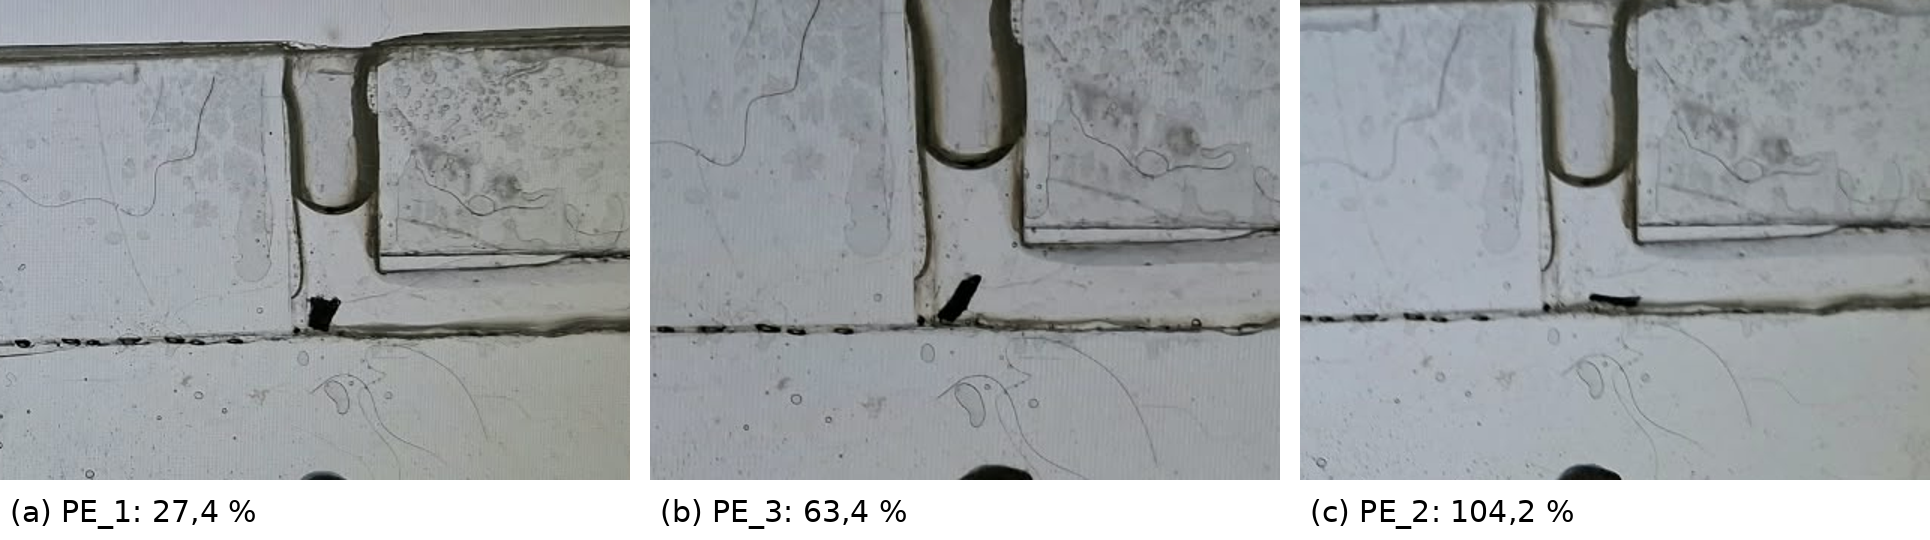
\includegraphics[width=\textwidth]{figuras/una_particula_orientacion.png}
  \caption{Posición de la partícula de 3~mm $\times$ 2~mm en los tres llenados, vista a
    contraluz: (a) de frente al haz en la esquina del canal; (b) en diagonal;
    (c) de canto sobre el borde del canal horizontal, sin detectarse.}
  \label{fig:una_particula}
\end{figure}

La partícula de 1~mm $\times$ 1~mm no se detectó en el único llenado realizado. Por ser
una sola medición, este resultado se toma como un indicio de que existe un tamaño mínimo
por debajo del cual la partícula no produce una caída suficiente, y no como un límite
de detección establecido. En uno de los intentos la partícula se movió fuera de la zona
de medición antes de terminar el calentamiento; la medición se canceló, se volvió a
ubicar la partícula y se repitió el llenado.

En conjunto, esta prueba muestra que lo decisivo es que la partícula quede justo dentro
del haz y de frente a él: la misma partícula pasó de bloquear el 73\,\% de la luz a no
detectarse solo por su posición. Esto también explica la mayor dispersión
observada en los llenados con PE durante la campaña.


% ---------------------------------------------------------------------
% BLOQUE B — FASE 5: EVALUACIÓN DEL CUMPLIMIENTO DE LOS OBJETIVOS
% ---------------------------------------------------------------------

\subsection{Evaluación del cumplimiento de los objetivos}

La Tabla~\ref{tab:criterios} compara los resultados con los criterios de aceptación
definidos en el anteproyecto, y la Tabla~\ref{tab:objetivos}, con los objetivos
específicos.

\begin{table}[htbp]
  \centering
  \caption{Cumplimiento de los criterios de aceptación del sistema.}
  \label{tab:criterios}
  \small
  \begin{tabular}{p{0.27\textwidth}p{0.49\textwidth}p{0.12\textwidth}}
    \hline
    Criterio & Evidencia & Estado \\
    \hline
    Señal estable sin saturación electrónica &
      Variación entre las 10 repeticiones de un llenado menor al 0,34\,\%; medición de
      cierre a 0,23\,\% y 0,78\,\% de la inicial; ninguna medición saturada en la campaña &
      Cumplido \\
    Repetibilidad aceptable &
      Variación entre llenados de agua limpia del 3,4\,\% (11 llenados, dos chips) &
      Cumplido \\
    Diferencia estadísticamente significativa entre muestra controlada y muestra con
      partículas &
      Prueba $t$ de Welch: $p = 1{,}8 \times 10^{-8}$; Mann-Whitney:
      $p = 8{,}2 \times 10^{-5}$; 22 de 22 llenados bien clasificados &
      Cumplido \\
    Funcionamiento continuo sin fallas durante las pruebas &
      La electrónica y el firmware operaron sin fallas en todas las sesiones. Los llenados
      afectados por filtraciones del chip se documentaron y se descartaron &
      Cumplido \\
    \hline
  \end{tabular}
\end{table}

\begin{table}[htbp]
  \centering
  \caption{Cumplimiento de los objetivos específicos.}
  \label{tab:objetivos}
  \small
  \begin{tabular}{p{0.17\textwidth}p{0.57\textwidth}p{0.14\textwidth}}
    \hline
    Objetivo & Evidencia & Estado \\
    \hline
    OE1. Sistema microfluídico con ventanas ópticas &
      Chip con canal en L y cámara con posición fija del chip, LED y fotodetector.
      Protocolo de llenado que redujo la variación del agua limpia al 3,4\,\%. El canal
      quedó en escala milimétrica (3~mm $\times$ 2~mm) por el tamaño de las partículas y el
      llenado es manual &
      Cumplido con limitaciones \\
    % Verificar que los números de tabla (4 y 5) coincidan con los del main.
    OE2. Caracterización y selección de la fuente &
      Comparación de longitudes de onda y de fuentes comerciales (Tablas 4 y 5), pruebas
      de distancia y de estabilidad térmica ($\tau \approx 69$~s); selección del LED
      TSAL4400 (940~nm) &
      Cumplido \\
    OE3. Adquisición y acondicionamiento de la señal &
      Fotodetector OPT101 (fotodiodo con amplificador de transimpedancia), conversión de 12 bits,
      modulación del LED y promedio de 1000 muestras por bloque (ruido del promedio
      reducido unas 31 veces), firmware con pruebas automáticas. Señal estable y sin
      saturación &
      Cumplido \\
    OE4. Validación frente a mediciones de referencia &
      Campaña de 22 llenados con fotografía a contraluz de cada uno como referencia;
      matriz de confusión con 22 aciertos de 22; precisión (repetibilidad) y confiabilidad
      cuantificadas &
      Cumplido \\
    \hline
  \end{tabular}
\end{table}

Respecto al objetivo general, el prototipo sí estima la presencia probable de partículas
compatibles con PE en agua cuando estas quedan en la zona de medición. Cada análisis toma
unos 3~min 20~s de medición más el tiempo de llenado, es decir, del orden de 6 a 7~min por
muestra. Los componentes del sistema son de bajo costo (Tabla~PENDIENTE de costos). La
portabilidad es parcial, porque la operación depende de un computador, y la aplicación en
campo todavía no se ha probado con muestras reales.


% ---------------------------------------------------------------------
% BLOQUE C — LIMITACIONES
% ---------------------------------------------------------------------

\subsection{Limitaciones}

\begin{itemize}
  \item \textbf{Zona de detección.} El prototipo solo detecta las partículas que quedan
    dentro del haz, y la caída depende de su orientación. Con una sola partícula se
    detectaron dos de tres llenados.
  \item \textbf{Tipo y tamaño de partícula.} Las pruebas se hicieron con partículas
    oscuras de 2~mm $\times$ 1~mm (campaña) y de 3~mm $\times$ 2~mm (prueba de una
    partícula), ubicadas en la zona de medición. Una partícula de 1~mm
    $\times$ 1~mm no se detectó, y no se probaron partículas transparentes o blancas,
    que son comunes en el ambiente.
  \item \textbf{Selectividad.} El sistema detecta cualquier objeto que atenúe la luz
    infrarroja; no identifica el polímero. Las burbujas producen caídas parecidas a las
    de una partícula, y se controlaron con el procedimiento de llenado.
  \item \textbf{Escala y manejo de la muestra.} El canal es de escala milimétrica, el
    llenado es manual y no hay flujo continuo.
  \item \textbf{Alineación.} Mover el fotodetector cambia mucho la señal; el montaje debe
    quedar fijo y cada sesión necesita su propia referencia con agua limpia.
  \item \textbf{Muestras y operación.} Solo se usó agua estéril de laboratorio, y la
    operación requiere un computador.
  \item \textbf{Tamaño de la muestra estadística.} Con 11 llenados por grupo, el
    intervalo de confianza del 95\,\% de la sensibilidad y la especificidad va del 71,5\,\%
    al 100\,\%.
\end{itemize}


% ---------------------------------------------------------------------
% BLOQUE D — CONCLUSIONES
% ---------------------------------------------------------------------

\section{Conclusiones}

\begin{enumerate}
  \item Se desarrolló un prototipo optoelectrónico de bajo costo, con un LED infrarrojo de
    940~nm, un fotodetector OPT101 y una Raspberry Pi Pico 2 W, que distingue el agua
    limpia del agua con partículas de polietileno de 2~mm $\times$ 1~mm ubicadas en la zona de
    medición. En 22 llenados con dos chips distintos, la señal de las muestras con PE
    bajó en promedio un 68\,\%, la diferencia fue estadísticamente significativa
    ($p = 1{,}8 \times 10^{-8}$) y todos los llenados quedaron bien clasificados con el
    umbral del 80\,\%.
  \item La parte electrónica resultó estable: la señal varió menos del 0,34\,\% dentro de
    un llenado y menos del 1\,\% a lo largo de una sesión. La mayor fuente de variación no
    fue la electrónica, sino el llenado del chip.
  \item Medir con el LED apagado y encendido, y restar ambos valores, hizo que la medición
    no se viera afectada por la luz ambiente: con un aumento del nivel de fondo de 22 a
    62~cuentas, los llenados de agua limpia siguieron alrededor del 100\,\% de la
    referencia.
  \item Las burbujas fueron el principal factor que podía confundirse con una partícula.
    Con un procedimiento de llenado definido, la variación del agua limpia bajó al
    3,4\,\% y la comparación entre grupos pasó de no significativa a contundente.
  \item La detección depende de que la partícula quede dentro del haz y de su orientación:
    la caída de señal corresponde a la sombra que la partícula proyecta. Por eso una sola
    partícula no siempre se detecta y una de 1~mm $\times$ 1~mm no se detectó en la prueba
    realizada.
  \item En consecuencia, el prototipo es viable como herramienta de análisis preliminar
    en condiciones controladas: es rápido (6 a 7~min por muestra), de bajo costo y sus
    resultados son repetibles. Para usarlo en campo todavía hace falta asegurar que las
    partículas pasen por la zona de medición, probar partículas transparentes y más
    pequeñas, trabajar con muestras reales y hacerlo independiente del computador.
\end{enumerate}


% ---------------------------------------------------------------------
% BLOQUE E — TRABAJO FUTURO
% ---------------------------------------------------------------------

\section{Trabajo futuro}

\begin{itemize}
  \item Incorporar topes o guías en el canal para que las partículas queden en la zona de
    medición sin ubicarlas a mano.
  \item Evaluar partículas transparentes, blancas y de menor tamaño, y otros polímeros.
  \item Probar muestras de agua reales y un sistema de flujo continuo con bomba.
  \item Estandarizar la fabricación del chip y reducir la escala del canal cuando se
    trabaje con partículas más pequeñas.
  \item Agregar una pantalla y alimentación por batería para operar sin computador.
  \item Ampliar el número de llenados para estimar con más precisión la sensibilidad y la
    especificidad.
  \item Explorar varias longitudes de onda o varios detectores para ganar selectividad y
    cubrir una zona de medición más amplia.
\end{itemize}


% ---------------------------------------------------------------------
% BLOQUE F — RESUMEN (borrador para completar)
% ---------------------------------------------------------------------

% Resumen
Los microplásticos están presentes en fuentes de agua de todo el mundo, pero su
detección depende de técnicas costosas y de laboratorio. En este trabajo se desarrolló
un prototipo de bajo costo para estimar la presencia probable de partículas compatibles
con microplásticos de polietileno (PE) en agua. El sistema usa un chip con un canal en L,
un LED infrarrojo de 940~nm, un fotodetector OPT101 y una Raspberry Pi Pico 2 W que mide
la luz transmitida con el LED apagado y encendido, y calcula la diferencia para eliminar
la luz ambiente. Se estableció un protocolo de llenado para controlar las burbujas y un
criterio de detección definido antes de las pruebas: la muestra se considera con
partículas si la señal cae por debajo del 80\,\% de la referencia con agua limpia. En una
campaña de 22 llenados con dos chips, las muestras con dos partículas de PE de 2~mm $\times$ 1~mm
redujeron la señal en promedio un 68\,\%, la diferencia con el agua limpia fue
estadísticamente significativa ($p = 1{,}8 \times 10^{-8}$) y los 22 llenados se
clasificaron correctamente. Una prueba complementaria mostró que la detección depende de
que la partícula quede dentro del haz y de su orientación. Se concluye que el prototipo
es viable como herramienta de análisis preliminar en condiciones controladas.

% Palabras clave: microplásticos, polietileno, detección óptica, infrarrojo,
% transmitancia, Lab-on-a-Chip, Raspberry Pi Pico.


% ---------------------------------------------------------------------
% BLOQUE G — FABRICACIÓN DEL CHIP (va donde el documento describe el chip
% en L; completa el pendiente "cómo se fabricó el canal").
% Figura opcional: figuras/chip_regla.png
% ---------------------------------------------------------------------

\subsubsection{Fabricación del chip}

El chip se fabricó con portaobjetos de vidrio para microscopio de 75~mm $\times$ 25~mm
y aproximadamente 1~mm de espesor, unidos con un adhesivo epóxico transparente
(Pegatanque). Está formado por
cuatro capas:

\begin{enumerate}
  \item \textbf{Base:} un portaobjetos completo.
  \item \textbf{Primera capa de paredes:} trozos de portaobjetos cortados con un cortador
    de vidrio y pegados sobre la base siguiendo una plantilla, de manera que entre ellos
    queda libre el canal en L.
  \item \textbf{Segunda capa de paredes:} igual a la anterior y pegada encima de ella,
    para darle más profundidad al canal.
  \item \textbf{Tapa:} otro portaobjetos completo, sin cortes.
\end{enumerate}

El chip terminado mide unos 75~mm $\times$ 25~mm, y el canal resultante, aproximadamente
3~mm de ancho por 2~mm de profundidad, un tamaño suficiente para que pasen las partículas
de prueba sin taparlo. Entre una capa y
la siguiente se esperó el tiempo de curado indicado por el fabricante del adhesivo, y la
plantilla permitió que los chips quedaran lo más parecidos posible entre sí
(Figura~\ref{fig:chip_regla}).

\begin{figure}[htbp]
  \centering
  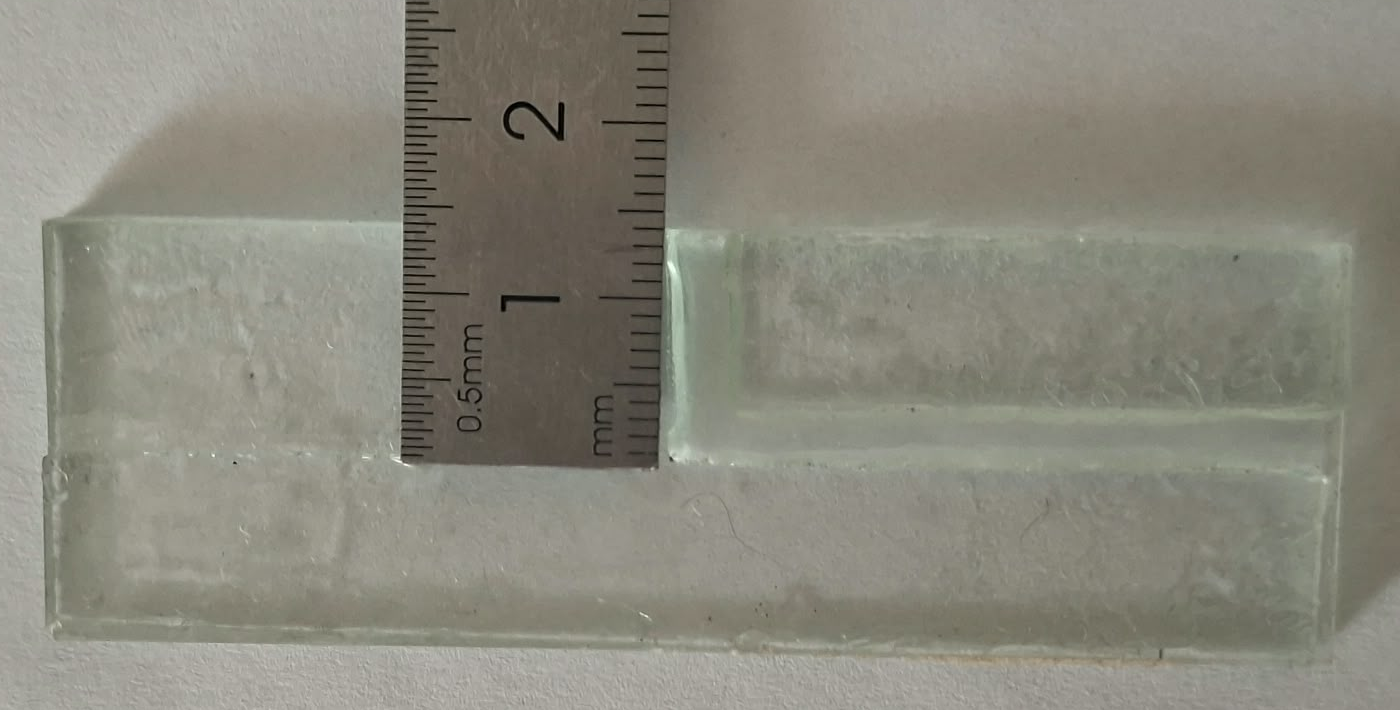
\includegraphics[width=0.7\textwidth]{figuras/chip_regla.png}
  \caption{Chip de vidrio con el canal en L, junto a una regla en milímetros.}
  \label{fig:chip_regla}
\end{figure}
